\documentclass[12pt,a4paper]{article}
\usepackage[utf8]{inputenc}
\usepackage[catalan]{babel}
\usepackage{graphicx}
\usepackage{geometry}
\usepackage{fancyhdr}
\usepackage{tabularx}
\usepackage{lastpage}
\usepackage{enumitem}
\usepackage{amsmath}
\usepackage{tikz}
\usepackage{tcolorbox}

% 1. MARGES I CAPÇALERA
\geometry{top=4cm, bottom=3cm, left=2cm, right=2cm, headheight=2.5cm}

\pagestyle{fancy}
% Pots descomentar les línies següents si tens els logos al teu projecte d'Overleaf
\fancyhead[L]{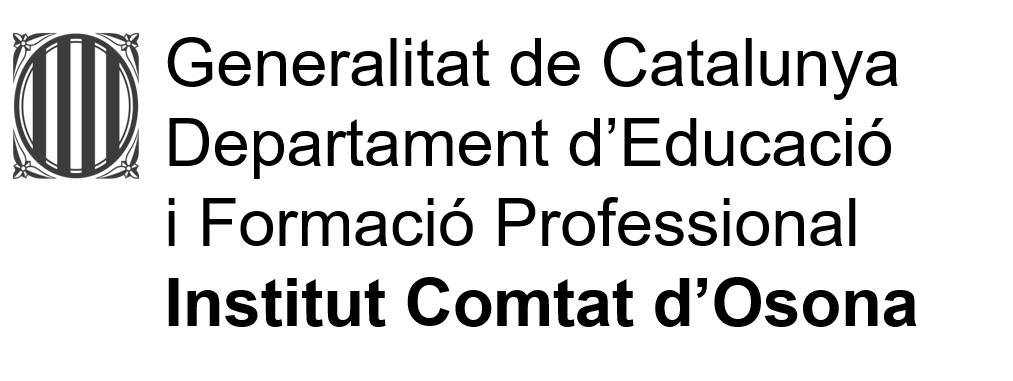
\includegraphics[height=1.8cm]{Logo_Departament.png}} 
\fancyhead[R]{
\includegraphics[height=1.8cm]{Logo_Institut.png}}
\fancyfoot[C]{Pàgina \thepage\ de \pageref{LastPage}}

\begin{document}

% --- CAPÇALERA D'IDENTIFICACIÓ ---
\begingroup
\renewcommand{\arraystretch}{2.2}
\begin{tabularx}{\textwidth}{|X|p{4cm}|}
    \hline
    \textbf{Nom i cognoms:} & \textbf{Grup:} \\ \hline
    \textbf{Activitat:} Fitxa 4: Resolució de problemes de Trigonometria & \textbf{Data:} \\ \hline
\end{tabularx}
\endgroup

\vspace{0.4cm}

\begin{tcolorbox}[colback=blue!5,colframe=blue!70!black,title=Recordatori ràpid: Fórmules Trigonomètriques]
\small
\textbf{En un triangle rectangle (SOH CAH TOA):} \\
$\sin(\alpha) = \dfrac{\text{Catet Oposat}}{\text{Hipotenusa}} \quad \quad \cos(\alpha) = \dfrac{\text{Catet Adjacent}}{\text{Hipotenusa}} \quad \quad \tan(\alpha) = \dfrac{\text{Catet Oposat}}{\text{Catet Adjacent}}$ \\[0.3cm]
\end{tcolorbox}


\textbf{1.} Una escala de bombers de 10 m de longitud està recolzada a la paret d'un edifici. L'angle que forma l'escala amb el terra és de 65º. A quina altura de l'edifici arriba l'escala? \\
\textit{El dibuix ja està fet. Només cal que triïs la raó trigonomètrica adequada i resolguis.}

\begin{minipage}{0.3\textwidth}
\begin{tikzpicture}[scale=0.6]
\draw[thick] (0,0) -- (3,0) -- (0,5) -- cycle;
\draw (0.3,0) -- (0.3,0.3) -- (0,0.3);
\draw (2.5,0) arc (180:121:0.5); \node at (2.0,0.4) {$65^\circ$};
\node at (2.4, 2.8) {Escala};
\node at (-0.8, 2.5) {Paret};
\node at (1.5, -0.4) {Terra};
\end{tikzpicture}
\end{minipage}
\begin{minipage}{0.65\textwidth}
\end{minipage}

\vspace{0.5cm}

\textbf{2.} Una altra escala es vol recolzar a una paret. Per motius de seguretat, sabem que la base de l'escala s'ha de situar exactament a 3 m de distància de la paret, i volem que formi un angle de 70º amb el terra. Quina longitud haurà de tenir aquesta escala?  \textit{Instrucció: Fes un dibuix i col·loca-hi les dades abans de resoldre!}

\vspace{3cm}

\textbf{3.} Un sender de gran recorregut puja una muntanya amb un pendent constant de 15º. Si un excursionista camina 500 metres pel sender, quina altura haurà guanyat respecte al punt de sortida? \\
\textit{Situa les dades en aquest esquema abans de resoldre.}

\begin{minipage}{0.3\textwidth}
\vspace{0.5cm}
\begin{tikzpicture}[scale=0.8]
\draw[thick] (0,0) -- (6,0) -- (6,2) -- cycle;
\draw (5.7,0) -- (5.7,0.3) -- (6,0.3);
\end{tikzpicture}
\end{minipage}
\begin{minipage}{0.65\textwidth}
\vspace{3.5cm}
\end{minipage}

\subsection*{Fase 2: Autonomia (plantejament propi)}
\textit{Fes el dibuix complet de cada situació per poder identificar el triangle.}

\vspace{0.5cm}

\textbf{4.} L'ombra d'una torre de comunicacions mesura 25 metres quan el sol es troba a una elevació de 55º sobre l'horitzontal. Quina és l'altura de la torre?

\vspace{4.5cm}


\textbf{5.} Una tirolina està lligada a un arbre a 10 metres d'alçada i arriba a una estaca clavada a terra. Si el cable de la tirolina fa 22 metres de llarg, quin angle de descens forma el cable amb l'arbre? 

\vspace{4.5cm}

\textbf{6.} \textbf{AN/AE} Un vigilant està dalt d'una torre costanera de 20 metres d'alçada. En línia recta cap a l'horitzó, veu dos vaixells de pesca:
\begin{itemize}
    \item El vaixell A el veu sota un angle de 40º amb l'horitzontal.
    \item El vaixell B el veu sota un angle de 20º amb l'horitzontal.
\end{itemize}
Quina distància hi ha entre el vaixell A i el vaixell B? \\
\textit{Pista: Hi ha dos triangles rectangles que fan servir la mateixa torre. Calcula la distància de la torre a cada vaixell per separat i després pensa com trobar la distància entre ells.}
\vspace{4.5cm}


\end{document}